Since the 1990s, quantum computing has become an important field of research in computer science. In 1998, we've seen the first quantum computer with 3 qubits and since then a lot of improvements and researches have been done to build a stable quantum computer. \newline

Let's anticipate the possible apogee of the quantum era and study how it could affect blockchains' security. We can watch some Youtube videos (see \cite{scienceEtonnante} and \cite{confTedEd}) as an introduction to quantum computers.

\section{What is Quantum computing ?}

Quantum computing differs from classic computing by the way it store and manipulate information. \newline

Let's have a quick reminder of how a classic computer works. \newline

They use bits to represent data, a bit can be either 0 or 1. Those two states are represented though an electrical signal. \newline

\begin{figure}[ht]
\centering
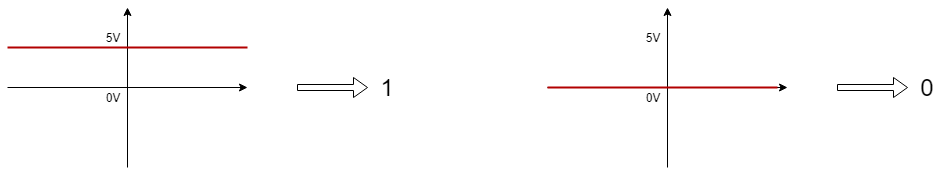
\includegraphics[width=14cm]{Figures/electricSignals}
\caption{Coding of a bit}
\end{figure}
\medskip

We process these signals with transistors to make logical gates, this is the basics of processors and computers architecture. To represent complex data, we create registers made of several bits. For example, a n-bits register can represent $2^n$ values / states. \newline

Now, what about quantum computing ? (see \cite{qubitWiki}) As the name suggests it, this new technology is based on quantum physics, the big difference with classic computers is that there isn't bits anymore but qubits or quantum bits. \newline

These qubits are not binary, either 0 or 1, but they exist in a superposition of 0 and 1. This is the superposition principle, we can understand it as probabilities so we commonly describe a qubit with the following formula: \newline

\begin{equation}
  \bra{x} = \alpha . \bra{0} + \beta . \bra{1}
\end{equation}
\medskip

where $\alpha$ is the probability for 0 and $\beta$ is the probability for 1. \newline

It's important to highlight that a quantum computer isn't an evolution of classic computers like clusters can be. A whole new technology is involved heading to a new way of representing and manipulating data. \newline

We won't go too far in the details about quantum physics and qubits but we can investigate two interesting questions. \newline

\paragraph{How do we physically build a qubit ?}

There are different possibilities to build a qubit, we need to use a two-level system, a system where a quantum superposition can exist. For example, we could use photons and light polarization, where we measure how much the light is vertically or horizontally polarized. \newline

One famous method is to use the spins of the electrons (see \cite{spinWiki}) where we measure the spin angular momentum to describe the quantum state of the electron. This spin is affected by the magnetic field around the particle. \newline

\begin{figure}[ht]
\centering
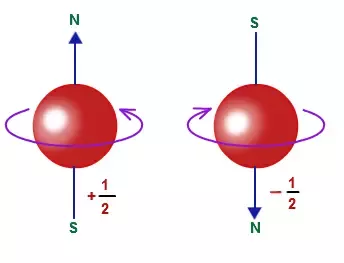
\includegraphics[width=6cm]{Figures/electronSpin}
\caption{Electron spin from \cite{spinNumber}}
\end{figure}
\medskip

These methods are more complicated than electric signals for classic bits, it's harder to keep the quantum bits stable. Researches are working on stability of qubits in order to build bigger computers.

\paragraph{How can we recover the state form a qubit ?}

Quantum computers follow a rule called "Wave function collapse", which says that a superposed state can't be known entirely, we can only measure it and so reduce it to one value.

This means that even if we have a $2^n$ superposed state, we will reduce it to one result. Then a quantum computer can be used only for specific problems with specifically designed algorithms like Grover algorithm. \newline

To conclude, a quantum computer will always be less polyvalent than its classical equivalent but it can be so much powerful for some specific problems. For example, it can be used for prime factorization, Peter Shor a scientist from Bell's lab found a quantum that could solve this problem. \newline
